\documentclass{beamer}
\usepackage{times, amsthm, amsmath, amssymb, cancel, changepage, graphicx, lipsum, fancyhdr, mathabx, enumitem,caption, subcaption}
\usetheme{CambridgeUS}
\usecolortheme{seagull}
\usefonttheme{serif}
\definecolor{navy}{RGB}{0, 0, 128} 
\setbeamercolor{frametitle}{fg=navy}
\setbeamercolor{title}{fg=navy}
\setbeamerfont{frametitle}{series=\bfseries}
\setbeamerfont{title}{series=\bfseries}

\title{Lecture 14: Change of Variables II}
\date{October 8, 2019}

\begin{document}
	
\frame{\titlepage}


\begin{frame}
\frametitle{Review: Change of Variables Formula}
\begin{figure}
	
	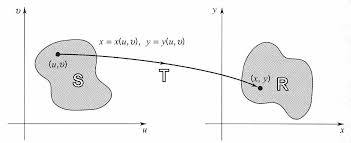
\includegraphics[width=.9\textheight]{vmap.jpg}\\
	\hspace*{10pt}\hbox{\thinspace{\tiny\itshape ksuweb.kenneshaw.edu}}
\end{figure}
If $J = \frac{\partial x}{\partial u} \frac{\partial y}{\partial v}-	\frac{\partial x}{\partial v}\frac{\partial y}{\partial u} \neq 0$,
$$\iint\limits_{R} f(x,y)dy\,dx = \iint\limits_{S} f[g(u,v),h(u,v)] |J| dv\,du$$


\end{frame}

\begin{frame}
\frametitle{A Bunch of Examples}
Examples:
\begin{itemize}
	\item[(1)] $T^{-1}: u=xy,v=xy^2$. Evaluate $\iint\limits_{R} y^2 dA$ where $R$ is bounded by the curves $xy=1,xy=2,xy^2=1,xy^2=2$.
	\item[(2)]$T: x=u/v, y=v$. Evaluate $\iint\limits_{R} xy \,dA$ where $R$ is the region in the first quadrant bounded by $y=x,y=3x,xy=1,xy=3$.
	\item[(3)]$T^{-1}: u=2x-y,v=x+y$. Evaluate $\iint\limits_{R} 6x-3y dA$ where $R$ is the region bounded by $2x-y=1,x+y=1,2x-y=3,x+y=3$.
	\item[(4)]$T^{-1}: u=y-x,v=y+x$. Evaluate $\iint\limits_{R} xy dA$ where $R$ is a square with verticies at $(0,1),(1,1),(2,0),(1,-1)$
\end{itemize}
\end{frame}


\begin{frame}
\frametitle{Polar Coordinates}
\begin{figure}

	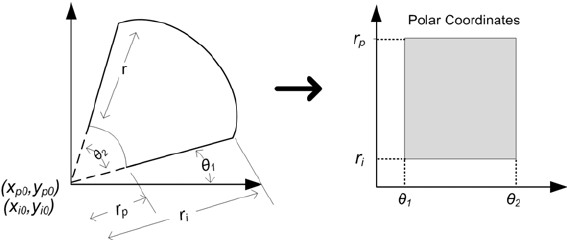
\includegraphics[height=.4\textheight]{polar.png}\\
	\hspace*{10pt}\hbox{\thinspace{\tiny\itshape researchgate.net}}
\end{figure}
Polar coordinates is just a specific type of transformation where $$T: x=r\cos \theta, y=r\sin \theta$$ Then the Jacobean is found by
$$M = \begin{bmatrix}
\frac{\partial x}{\partial u} & 	\frac{\partial x}{\partial v}\\
\frac{\partial y}{\partial u} & 	\frac{\partial y}{\partial v}
\end{bmatrix}  = \begin{bmatrix} \cos \theta & -r\sin \theta \\ \sin \theta & r\cos \theta \end{bmatrix} \mbox{ giving } J=|M| = r\cos^2 \theta + r\sin^2 \theta = r$$

\end{frame}


\begin{frame}
\frametitle{Polar Coordinates}
\textbf{Examples:}
\begin{itemize}
	\item[(a)] Evaluate $\iint\limits_{R} e^{x^2+y^2} dy\,dx$ where $R$ is the unit circle.
	\item[(b)] Evaluate $\int_{-\infty}^\infty e^{-x^2/2}dx$.
\end{itemize}
\end{frame}


\begin{frame}
\frametitle{Triple Integrals \& Change of Variables}
$T$ now maps region $S$ in the $(u,v,w)$ space onto $R$ in the $(x,y,z)$ space via
$$T: x=g(u,v,w),y=g(u,v,w),z=k(u,v,w)$$
This gives a Jacobean of 
$$J=|M| = \Bigg|\begin{matrix}
\frac{\partial x}{\partial u} & \frac{\partial x}{\partial v} & \frac{\partial x}{\partial w}\\
\frac{\partial y}{\partial u} & \frac{\partial y}{\partial v} & \frac{\partial y}{\partial w}\\
\frac{\partial z}{\partial u} & \frac{\partial z}{\partial v} & \frac{\partial z}{\partial w}
\end{matrix} \Bigg|$$
And the follow change of variables formula
$$\iiint\limits_{R} f(x,y,z)dV = \iiint\limits_{S} f(g(u,v,w),h(u,v,w),k(u,v,w)) |J| du\, dv\, dw$$
\end{frame}

\end{document}
